\documentclass{beamer}



\usepackage[utf8]{inputenc}
\usepackage[english]{babel}

\usepackage{amsmath}
\usepackage{amssymb}
\usepackage{amsfonts}
\newcommand\eqbydef{\mathrel{\overset{\makebox[0pt]{\mbox{\normalfont\tiny\sffamily def}}}{=}}}

\usepackage{xcolor}
\usepackage{graphicx}
\usepackage{float}
\usepackage{enumerate}

\usepackage{xspace}
\makeatletter
\DeclareRobustCommand\onedot{\futurelet\@let@token\@onedot}
\def\@onedot{\ifx\@let@token.\else.\null\fi\xspace}
\def\eg{{e.g}\onedot}
\def\Eg{{E.g}\onedot}
\def\ie{{i.e}\onedot}
\def\Ie{{I.e}\onedot}
\def\etc{{etc}\onedot}
\def\etal{{et~al}\onedot}
\def\WLOG{w.l.o.g\onedot}

\usepackage{tikz}
\usetikzlibrary{arrows,decorations.pathmorphing,positioning,fit,trees,shapes}

\usepackage{newalg}
\newtheorem{Algorithm}{Algorithm}
\floatstyle{ruled}
\newfloat{Algorithm}{thp}{lop}
\floatname{Algorithm}{Algorithm}
\restylefloat{table}



\title{Difference Logic \\
    {\large Satisfiability Checking Seminar}
}
\author{Alex Ryndin \\ Supervisor: Gereon Kremer}
\date{WS 2016/2017}



\begin{document}
    \maketitle



    \begin{frame}
        \frametitle{Outline}
        \begin{itemize}
            \item Main Literature
            \item Difference Logic
            \item Example Problem: Job Scheduling
            \item SAT Checking of Propositional Logic
            \item SAT Checking of Difference Logic
            \item Constraint Graph
            \item Negative Cycles in a Constraint Graph
            \item How to Find a Negative Cycle in a Graph
            \item Goldberg-Radzik Heuristic
            \item SAT Checking Algorithm for Difference Logic (Sketch)
            \item Conclusion
        \end{itemize}
    \end{frame}



    \begin{frame}
        \frametitle{Main Literature}
        \begin{itemize}
            \item \textcolor{blue}{[Cotton \etal 2004]}
            Scott Cotton, Eugene Asarin, Oded Maler
            and Peter Niebert. \textbf{``Some progress in
            satisfiability checking for difference logic``}.
            In Formal Techniques, Modelling and Analysis
            of Timed and Fault-Tolerant Systems,
            pages 263--276. Springer, 2004.
            \item \textcolor{blue}{[Goldberg+Radzik 1993]}
            Andrew V. Goldberg and Tomasz Radzik.
            \textbf{``A heuristic improvement of
                the Bellman-Ford algorithm``}.
            Applied Mathematics Letters, 6(3):3–6, 1993.
            \item \textcolor{blue}{[Cormen \etal 2009]}
            Thomas H. Cormen, Charles E. Leiserson,
            Ronald L. Rivest and Clifford Stein.
            \textbf{``Introduction to algorithms``}.
            MIT press, third edition, 2009.
            \\
            Note: the chapter 24
            \textbf{``Single-Source Shortest Paths``}
            is relevant for the topic.
        \end{itemize}
    \end{frame}



    \begin{frame}
        \frametitle{Difference Logic}
        \begin{itemize}
            \item Difference logic (DL) is a special case of
            linear arithmetic (LA) logic.
            \item It is a Propositional Logic (PL)
            enhanced with constraints of the following form:
            \begin{equation}
                x - y \prec c
            \end{equation}
            where $ x,y $ are variables, $ c $ is a constant
            and $ \prec \in \{ <, \le \} $ is a comparison operator.
            \item $ x,y,c $ can be defined either over
            Integers $ \mathbb{Z} $
            or over Reals $ \mathbb{R} $.
        \end{itemize}
    \end{frame}




    \begin{frame}
        \frametitle{Difference Logic}
        \begin{itemize}
            \item A couple of examples:
        \end{itemize}
        \begin{equation}
            \phi_1 = (p \lor q)
            \land (p \rightarrow (u - v < 3.3))
            \land (q \rightarrow (v - w < -5.15))
        \end{equation}
        \begin{equation}
            \begin{aligned}
                \phi_2 &= (u-v < 1) \land (v-w < 5) \\
                & \land (w-x \leq -3) \land (x-y < 1) \\
                & \land (y-z \leq -5) \land (y-v \leq 0) \\
            \end{aligned}
        \end{equation}
        \begin{equation}
            \begin{aligned}
                \phi_3 &= (u-v < 1) \land (v-w < 5) \\
                & \land (w-x \leq -3) \land (x-y < -3) \\
                & \land (y-z \leq -5) \land (y-w < 4) \\
            \end{aligned}
        \end{equation}
    \end{frame}




    \begin{frame}
        \frametitle{Difference Logic. Special cases}
        \begin{itemize}
            \item $ x < c \;\; \Leftrightarrow \;\; x - 0 < c \;\; \Leftrightarrow \;\; x - zero < c $
            where $ zero $ is a
            \textcolor{blue}{special variable}
            which, however, \textcolor{blue}{does not change}
            the algorithm for deciding SAT of DL formula.
            \item $ x \ge c \;\; \Leftrightarrow \;\; -x \le -c \;\; \Leftrightarrow \;\; 0 - x \le -c \;\; \Leftrightarrow \;\; zero - x \le -c $
            \item $ x \neq c \;\; \Leftrightarrow \;\; ((x < c) \lor (x > c)) $
            and then see above
            \item $ x = c \;\; \Leftrightarrow \;\; \neg ((x < c) \lor (x > c)) $
            and then see above
            \item An example:
            \begin{equation*}
                \begin{aligned}
                    (v = -3) \\
                    (\neg ((v < -3) \lor (v > -3))) \\
                    (\neg ((v < -3) \lor (-v < 3))) \\
                    (\neg ((v-0 < -3) \lor (0-v < 3))) \\
                    (\neg ((v-zero < -3) \lor (zero-v < 3))) \\
                \end{aligned}
            \end{equation*}
        \end{itemize}
    \end{frame}




    \begin{frame}
        \frametitle{Example Problem: Job Scheduling}
        \begin{figure}[htb]
            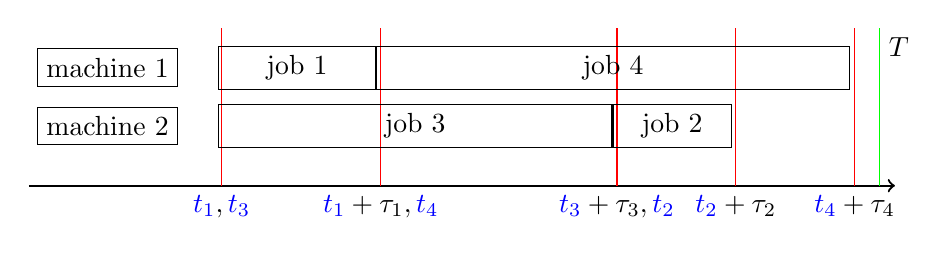
\begin{tikzpicture}
                \draw[thick,->] (-1,-1.5) -- (10,-1.5);

                \draw[color=red] (1.45,0.5) -- (1.45,-1.5);
                \draw (1.45,-1.5) -- (1.45,-1.5)
                            node[anchor=north] {$ \textcolor{blue}{t_1}, \textcolor{blue}{t_3} $};

                \draw[color=red] (3.47,0.5) -- (3.47,-1.5);
                \draw (3.47,-1.5) -- (3.47,-1.5)
                            node[anchor=north] {$ \textcolor{blue}{t_1}+\tau_1, \textcolor{blue}{t_4} $};

                \draw[color=red] (6.47,0.5) -- (6.47,-1.5);
                \draw (6.47,-1.5) -- (6.47,-1.5)
                            node[anchor=north] {$ \textcolor{blue}{t_3}+\tau_3, \textcolor{blue}{t_2} $};

                \draw[color=red] (7.98,0.5) -- (7.98,-1.5);
                \draw (7.98,-1.5) -- (7.98,-1.5)
                            node[anchor=north] {$ \textcolor{blue}{t_2}+\tau_2 $};

                \draw[color=red] (9.49,0.5) -- (9.49,-1.5);
                \draw (9.49,-1.5) -- (9.49,-1.5)
                            node[anchor=north] {$ \textcolor{blue}{t_4}+\tau_4 $};

                \draw[color=green] (9.8,0.5) -- (9.8,-1.5);
                \draw (9.8,0.5) -- (9.8,0.5)
                            node[anchor=north west] {$ T $};

                \node [draw] (m1) at (0,0) {machine 1};
                \node [draw, below = 0.25cm of m1] (m2) {machine 2};
                \node [draw, minimum width=2cm,
                        right = 0.5cm of m1]
                                        (job1) {job 1};
                \node [draw, minimum width=6cm,
                        right = 0cm of job1]
                                        (job4) {job 4};
                \node [draw, minimum width=5cm,
                        right = 0.5cm of m2]
                                        (job3) {job 3};
                \node [draw, minimum width=1.5cm,
                        right = 0cm of job3]
                                        (job2) {job 2};
            \end{tikzpicture}
        \end{figure}
    \begin{itemize}
        \item $ \textcolor{blue}{p_{mj}} = True $
        if job $ j $ is scheduled
        on machine $ m $:
        \\
        e.g. $ \textcolor{blue}{p_{11}} = \textcolor{blue}{p_{14}} = \textcolor{blue}{p_{23}} = \textcolor{blue}{p_{22}} = True $
        for the figure above
        \item job $ i $ starts at $ \textcolor{blue}{t_i} $
        and lasts $ \tau_i $
        \item a machine cannot process two or more jobs
        simultaneously:
        \\
        $ (\textcolor{blue}{p_{mi}} \land \textcolor{blue}{p_{mj}}) \rightarrow ((\textcolor{blue}{t_i} + \tau_i \le \textcolor{blue}{t_j}) \lor (\textcolor{blue}{t_j} + \tau_j \le \textcolor{blue}{t_i})) \quad \Leftrightarrow $
        \\
        $ (\textcolor{blue}{p_{mi}} \land \textcolor{blue}{p_{mj}}) \rightarrow ((\textcolor{blue}{t_i} - \textcolor{blue}{t_j} \le -\tau_i) \lor (\textcolor{blue}{t_j} - \textcolor{blue}{t_i} \le -\tau_j)) $
        \item the overall processing time should not exceed $ T $:
        \\
        $ \textcolor{blue}{t_i} + \tau_i \le T \quad \Leftrightarrow \quad \textcolor{blue}{t_i} - 0 \le T -\tau_i $
    \end{itemize}
    \end{frame}



    \begin{frame}
        \frametitle{Example Problem: Job Scheduling}
        \begin{equation*}
            \begin{aligned}
                \phi &= \bigwedge_{j=1}^{4} (p_{1j} \lor p_{2j}) \quad \land \\
                & \mathrm{each \; task \; is \; executed \; on \; at \; least \; one \; machine} \\
                & \bigwedge_{j=1}^{4} ((p_{1j} \rightarrow \neg p_{2j}) \land (p_{2j} \rightarrow \neg p_{1j})) \quad \land \\
                & \mathrm{each \; task \; can \; be \; scheduled \; on \; one \; machine\; only } \\
                & \bigwedge_{j=1}^{4} (t_j \ge 0) \; \land \; \bigwedge_{j=1}^{4} (t_j \le T-\tau_j) \quad \land \\
                & \mathrm{general \; time \; constraints} \\
                & \bigwedge_{m=1}^{2} \bigwedge_{i=1}^{3} \bigwedge_{j=i+1}^{4} ((p_{mi} \land p_{mj}) \rightarrow ((t_i-t_j \le -\tau_i) \lor (t_j-t_i \le -\tau_j))) \\
                & \mathrm{no \; time \; overlap \; rule} \\
            \end{aligned}
        \end{equation*}
    \end{frame}



    \begin{frame}
        \frametitle{SAT Checking of Propositional Logic}
        \begin{columns}[T]
            \begin{column}{.4\textwidth}
                \begin{equation*}
                    \phi = (a \lor b) \land (b \lor c) \land (c \lor a) \land \dots
                \end{equation*}
                SAT checking = intelligent search in the model space.
                The model space can be represented as a tree.
            \end{column}
            \begin{column}{.4\textwidth}
                \begin{figure}[htb]
                    \resizebox {1.33\linewidth} {!} {
                        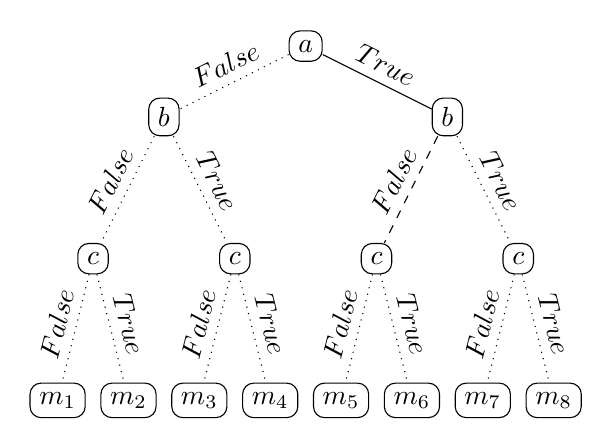
\begin{tikzpicture}[scale=0.9,state/.style={draw, rounded corners, fill=none,text centered, text=black}]
    \node[state] (n1) at (3.5, 5) {$a$};

    \node[state] (n2) at (1.5, 4) {$b$};
    \node[state] (n3) at (5.5, 4) {$b$};
    
    \node[state] (n4) at (0.5, 2) {$c$};
    \node[state] (n5) at (2.5, 2) {$c$};
    \node[state] (n6) at (4.5, 2) {$c$};
    \node[state] (n7) at (6.5, 2) {$c$};

    \node[state] (n8) at (0, 0) {$m_1$};
    \node[state] (n9) at (1, 0) {$m_2$};
    \node[state] (n10) at (2, 0) {$m_3$};
    \node[state] (n11) at (3, 0) {$m_4$};
    \node[state] (n12) at (4, 0) {$m_5$};
    \node[state] (n13) at (5, 0) {$m_6$};
    \node[state] (n14) at (6, 0) {$m_7$};
    \node[state] (n15) at (7, 0) {$m_8$};

    \path[every node/.style={sloped,anchor=south,auto=false}]
        (n1) edge[dotted] node {$False$} (n2)
        (n1) edge node {$True$} (n3)

        (n2) edge[dotted] node {$False$} (n4)
        (n2) edge[dotted] node {$True$} (n5)
        (n3) edge[dashed] node {$False$} (n6)
        (n3) edge[dotted] node {$True$} (n7)

        (n4) edge[dotted] node {$False$} (n8)
        (n4) edge[dotted] node {$True$} (n9)
        (n5) edge[dotted] node {$False$} (n10)
        (n5) edge[dotted] node {$True$} (n11)
        (n6) edge[dotted] node {$False$} (n12)
        (n6) edge[dotted] node {$True$} (n13)
        (n7) edge[dotted] node {$False$} (n14)
        (n7) edge[dotted] node {$True$} (n15);
\end{tikzpicture}

                    }
                \end{figure}
            \end{column}
        \end{columns}
    \end{frame}



    \begin{frame}
        \frametitle{SAT Checking of Propositional Logic}
        \begin{figure}[htb]
            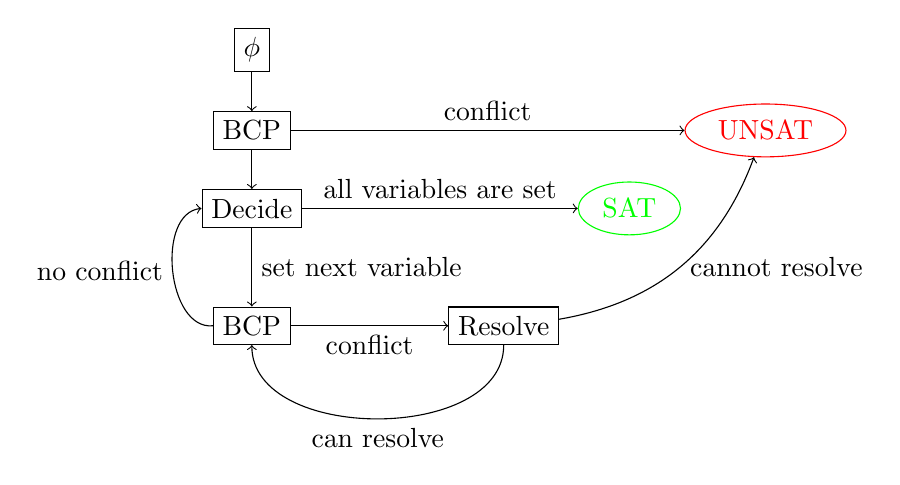
\begin{tikzpicture}
            \tikzstyle{block} = [draw, rectangle]

            \node [block] (formula) {$ \phi $};
            \node [block, below = 0.5cm of formula] (BCP) {BCP};
            \node [draw, ellipse, color=red, right = 5cm of BCP] (unsat) {UNSAT};
            \node [block, below = 0.5cm of BCP] (decide) {Decide};
            \node [draw, ellipse, color=green, right = 3.5cm of decide] (sat) {SAT};
            \node [block, below = 1cm of decide] (BCP2) {BCP};
            \node [block, right = 2cm of BCP2] (resolve) {Resolve};
            \draw[->] (formula) -- (BCP);
            \draw [->] (BCP) -- node[anchor=south] {conflict} (unsat);
            \draw [->] (BCP) -- (decide);
            \draw [->] (decide) -- node[anchor=south] {all variables are set} (sat);
            \draw [->] (decide) -- node[anchor=west] {set next variable} (BCP2);
            \draw [->] (BCP2) -- node[anchor=north] {conflict} (resolve);
            \draw [->] (BCP2) edge[bend left=90] node[anchor=east] {no conflict} (decide);
            \draw [->] (resolve) edge[bend right=30] node[anchor=west] {cannot resolve} (unsat);
            \draw [->] (resolve) edge[bend left=90] node[anchor=north] {can resolve} (BCP2);
            \end{tikzpicture}
        \end{figure}
    \end{frame}



    \begin{frame}
        \frametitle{SAT Checking of Difference Logic}
        \begin{figure}[htb]
            \resizebox {0.55\linewidth} {!} {
                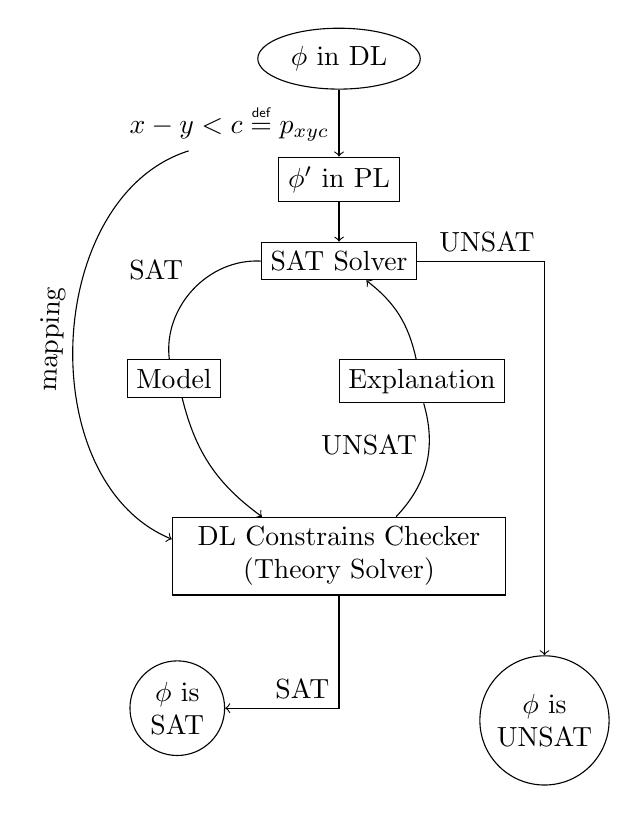
\begin{tikzpicture}

\tikzstyle{block} = [draw, rectangle]

\node [draw, ellipse] (dl) {$ \phi $ in DL};
\node [block, below = 0.85cm of dl] (pl) {$ \phi' $ in PL};
\node [block, below = 0.5cm of pl] (sat-solver) {SAT Solver};
\node [block, below left = 1cm and 0.5cm of sat-solver] (model) {Model};
\node [block, below right = 1cm and -1cm of sat-solver] (explanation) {Explanation};
\node [block, below = 3cm of sat-solver, text width=4cm, align=center] (theory-solver) {DL Constrains Checker (Theory Solver)};
\node [draw, circle, inner sep=0pt, text width=1cm, align=center, below left = 1cm and -0.5cm of theory-solver] (sat) {$ \phi $ is SAT};
\node [draw, circle, inner sep=0pt, text width=1.5cm, align=center, below right = 1cm and -0.1cm of theory-solver] (unsat) {$ \phi $ is UNSAT};

\draw [->] (dl) -- node[anchor=east, name=substitution] {$ x - y < c \eqbydef p_{xyc} $} (pl);
\draw [->] (pl) -- (sat-solver);
\draw [->] (substitution) edge[bend right=70] node[anchor=south, sloped] {mapping} (theory-solver);
\draw [-] (sat-solver.west) edge[bend right=50] node[anchor=south east] {SAT} (model);
\draw [->] (model) edge[bend right=20] (theory-solver);
\draw [->] (sat-solver) -| node[anchor=south east] {UNSAT} (unsat);
\draw [-] (theory-solver) edge[bend right=30] node[anchor=south east] {UNSAT} (explanation);
\draw [->] (explanation) edge[bend right=20] (sat-solver);
\draw [->] (theory-solver) |- node[anchor=south east] {SAT} (sat);
\end{tikzpicture}
            }
            \caption{Lazy approach}
        \end{figure}
    \end{frame}



    \begin{frame}
        \frametitle{SAT Checking of Difference Logic}
        \begin{figure}[htb]
            \resizebox {0.9\linewidth} {!} {
                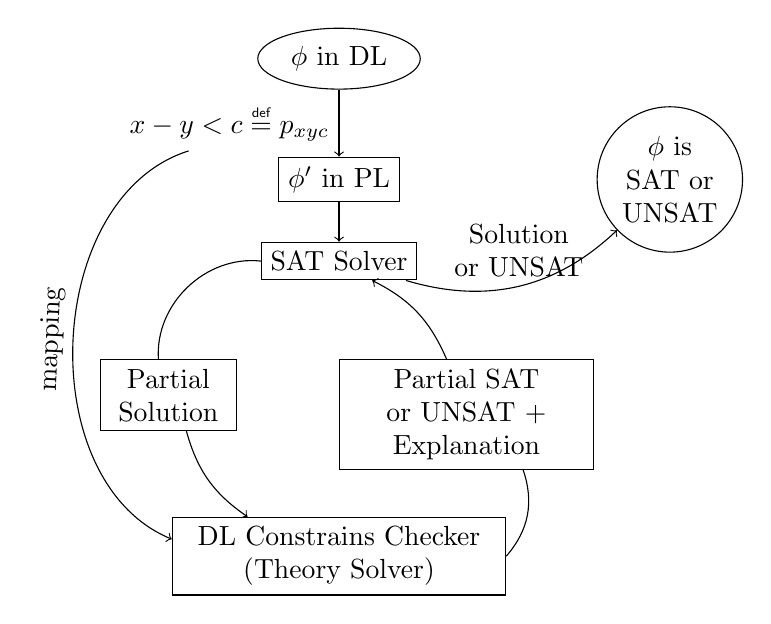
\begin{tikzpicture}

\tikzstyle{block} = [draw, rectangle]

\node [draw, ellipse] (dl) {$ \phi $ in DL};
\node [block, below = 0.85cm of dl] (pl) {$ \phi' $ in PL};
\node [block, below = 0.5cm of pl] (sat-solver) {SAT Solver};
\node [block, below left = 1cm and 0.3cm of sat-solver, text width=1.5cm, align=center] (model) {Partial Solution};
\node [block, below right = 1cm and -1cm of sat-solver, text width=3cm, align=center] (explanation) {Partial SAT or UNSAT + Explanation};
\node [block, below = 3cm of sat-solver, text width=4cm, align=center] (theory-solver) {DL Constrains Checker (Theory Solver)};
\node [draw, circle, inner sep=0pt, text width=1.5cm, align=center, right = 2.5cm of pl] (sat) {$ \phi $ is SAT or UNSAT};

\draw [->] (dl) -- node[anchor=east, name=substitution] {$ x - y < c \eqbydef p_{xyc} $} (pl);
\draw [->] (pl) -- (sat-solver);
\draw [->] (substitution) edge[bend right=70] node[anchor=south, sloped] {mapping} (theory-solver);
\draw [-] (sat-solver.west) edge[bend right=50] (model);
\draw [->] (model) edge[bend right=20] (theory-solver);
\draw [-] (theory-solver.east) edge[bend right=30] (explanation);
\draw [->] (explanation) edge[bend right=20] (sat-solver);
\draw [->] (sat-solver) edge[bend right=30] node[anchor=south, text width=2cm, align=center] {Solution or UNSAT} (sat);
\end{tikzpicture}
            }
            \caption{Incremental approach}
        \end{figure}
    \end{frame}



    \begin{frame}
        \frametitle{Constraint Graph}
        \begin{columns}[T]
            \begin{column}{.4\textwidth}
                \begin{figure}[htb]
                    \resizebox {\linewidth} {!} {
                        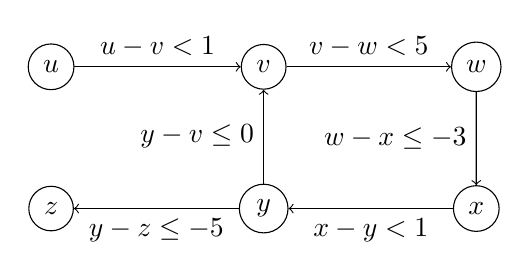
\begin{tikzpicture}[scale=0.9,state/.style={draw, circle, fill=none,text centered, text=black}]
    \node[state] (u) at (0, 2) {$u$};
    \node[state] (v) at (3, 2) {$v$};
    \node[state] (w) at (6, 2) {$w$};
    \node[state] (x) at (6, 0) {$x$};
    \node[state] (y) at (3, 0) {$y$};
    \node[state] (z) at (0, 0) {$z$};
    \draw [->] (u) -- node[anchor=south] {$ u-v < 1 $} (v);
    \draw [->] (v) -- node[anchor=south] {$ v-w < 5 $} (w);
    \draw [->] (w) -- node[anchor=east] {$ w-x \leq -3 $} (x);
    \draw [->] (x) -- node[anchor=north] {$ x-y < 1 $} (y);
    \draw [->] (y) -- node[anchor=north] {$ y-z \leq -5 $} (z);
    \draw [->] (y) -- node[anchor=east] {$ y-v \leq 0 $} (v);
\end{tikzpicture}

                    }
                \end{figure}
                \begin{equation*}
                    \begin{aligned}
                    \phi_2 &= (u-v < 1) \\
                    & \land (v-w < 5) \\
                    & \land (w-x \leq -3) \\
                    & \land (x-y < 1) \\
                    & \land (y-z \leq -5) \\
                    & \land (y-v \leq 0) \\
                    \end{aligned}
                \end{equation*}
            \end{column}
            \begin{column}{.4\textwidth}
                \begin{figure}[htb]
                    \resizebox {1.33\linewidth} {!} {
                        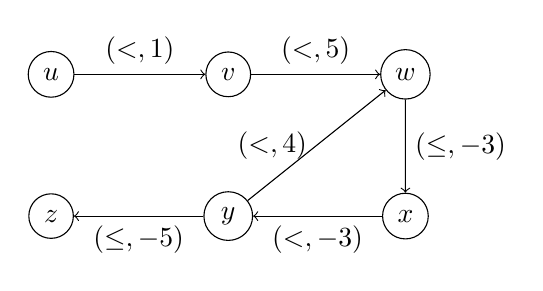
\begin{tikzpicture}[scale=0.9,state/.style={draw, circle, fill=none,text centered, text=black}]
    \node[state] (u) at (0, 2) {$u$};
    \node[state] (v) at (2.5, 2) {$v$};
    \node[state] (w) at (5, 2) {$w$};
    \node[state] (x) at (5, 0) {$x$};
    \node[state] (y) at (2.5, 0) {$y$};
    \node[state] (z) at (0, 0) {$z$};
    \draw [->] (u) -- node[anchor=south] {$ (<,1) $} (v);
    \draw [->] (v) -- node[anchor=south] {$ (<,5) $} (w);
    \draw [->] (w) -- node[anchor=west] {$ (\leq,-3) $} (x);
    \draw [->] (x) -- node[anchor=north] {$ (<,-3) $} (y);
    \draw [->] (y) -- node[anchor=north] {$ (\leq,-5) $} (z);
    \draw [->] (y) -- node[anchor=east] {$ (<,4) $} (w);
\end{tikzpicture}

                    }
                \end{figure}
                \begin{equation*}
                    \begin{aligned}
                    \phi_3 &= (u-v < 1) \\
                    & \land (v-w < 5) \\
                    & \land (w-x \leq -3) \\
                    & \land (x-y < -3) \\
                    & \land (y-z \leq -5) \\
                    & \land (y-w < 4) \\
                    \end{aligned}
                \end{equation*}
            \end{column}
        \end{columns}
        \begin{equation*}
            \Gamma = (V, E, weight, op)
        \end{equation*}
    \end{frame}
    

    
    \begin{frame}
        \frametitle{Negative Cycles in a Constraint Graph}
        \begin{columns}[T]
            \begin{column}{.4\textwidth}
                Negative cycle
                $ x \rightarrow y \rightarrow w \rightarrow x $
                \begin{equation*}
                    \begin{aligned}
                    x - y & < -3 \\
                    y - w & < \;\;\; 4 \\
                    w - x & \leq -3 \\
                    \hline
                    \textcolor{red}{0} \; & \textcolor{red}{< -2}
                    \end{aligned}
                    \end{equation*}
                    \textcolor{red}{A conflict!}
            \end{column}
            \begin{column}{.4\textwidth}
                \begin{figure}[htb]
                    \resizebox {1.33\linewidth} {!} {
                        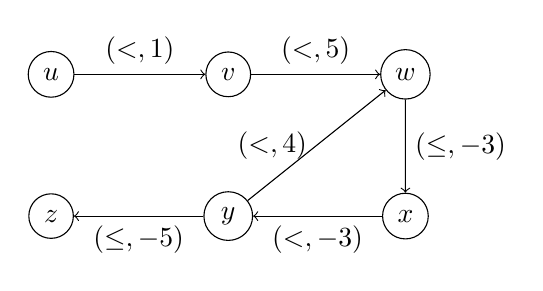
\begin{tikzpicture}[scale=0.9,state/.style={draw, circle, fill=none,text centered, text=black}]
    \node[state] (u) at (0, 2) {$u$};
    \node[state] (v) at (2.5, 2) {$v$};
    \node[state] (w) at (5, 2) {$w$};
    \node[state] (x) at (5, 0) {$x$};
    \node[state] (y) at (2.5, 0) {$y$};
    \node[state] (z) at (0, 0) {$z$};
    \draw [->] (u) -- node[anchor=south] {$ (<,1) $} (v);
    \draw [->] (v) -- node[anchor=south] {$ (<,5) $} (w);
    \draw [->] (w) -- node[anchor=west] {$ (\leq,-3) $} (x);
    \draw [->] (x) -- node[anchor=north] {$ (<,-3) $} (y);
    \draw [->] (y) -- node[anchor=north] {$ (\leq,-5) $} (z);
    \draw [->] (y) -- node[anchor=east] {$ (<,4) $} (w);
\end{tikzpicture}

                    }
                \end{figure}
                \begin{equation*}
                \begin{aligned}
                \phi_3 &= (u-v < 1) \\
                & \land (v-w < 5) \\
                & \land (w-x \leq -3) \\
                & \land (x-y < -3) \\
                & \land (y-z \leq -5) \\
                & \land (y-w < 4) \\
                \end{aligned}
                \end{equation*}
            \end{column}
        \end{columns}
    \end{frame}
    
    
    
    \begin{frame}
        \frametitle{How to Find a Negative Cycle in a Graph}
        \begin{itemize}
            \item First idea: enumerate all cycles
            \begin{itemize}
                \item and check if they are negative \\
                ($ 0 \prec c $ conflict clause where $ c < 0$
                and $ \prec \in \{ <, \le \} $)
                \item or they have zero weight and an edge with a strict inequality \\
                ($ 0 < 0 $ conflict clause)
            \end{itemize}
            \item Johnson algorithm solves the cycles enumeration problem
            \begin{itemize}
                \item $ O((|V|+|E|) \cdot (C+1)) $ time complexity,
                where $ C $ is number of elementary cycles
            \end{itemize}
            \item \textcolor{blue}{Any problems with this approach?}
        \end{itemize}
    \end{frame}



    \begin{frame}
        \frametitle{How to Find a Negative Cycle in a Graph}
        \begin{figure}[htb]
            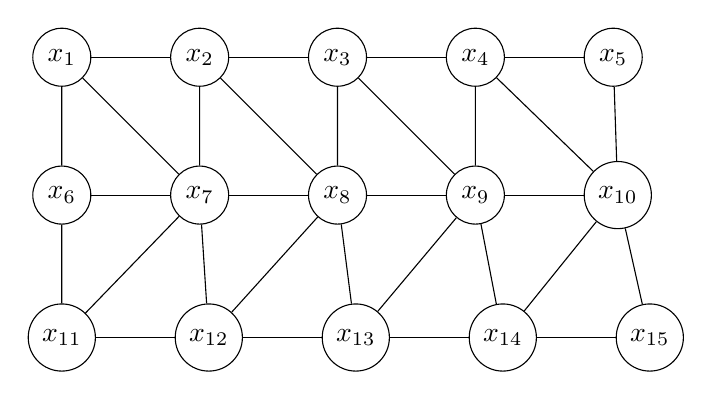
\begin{tikzpicture}
            \node [draw, circle] (x1) {$ x_1 $};
            \node [draw, circle, right = of x1] (x2) {$ x_2 $};
            \node [draw, circle, right = of x2] (x3) {$ x_3 $};
            \node [draw, circle, right = of x3] (x4) {$ x_4 $};
            \node [draw, circle, right = of x4] (x5) {$ x_5 $};
            \draw (x1) -- (x2) -- (x3) -- (x4) -- (x5);
            \node [draw, circle, below = of x1] (x6) {$ x_6 $};
            \node [draw, circle, right = of x6] (x7) {$ x_7 $};
            \node [draw, circle, right = of x7] (x8) {$ x_8 $};
            \node [draw, circle, right = of x8] (x9) {$ x_9 $};
            \node [draw, circle, right = of x9] (x10) {$ x_{10} $};
            \draw (x6) -- (x7) -- (x8) -- (x9) -- (x10);
            \draw (x6) -- (x1) -- (x7) -- (x2) -- (x8) -- (x3) -- (x9) -- (x4) -- (x10) -- (x5);
            \node [draw, circle, below = of x6] (x11) {$ x_{11} $};
            \node [draw, circle, right = of x11] (x12) {$ x_{12} $};
            \node [draw, circle, right = of x12] (x13) {$ x_{13} $};
            \node [draw, circle, right = of x13] (x14) {$ x_{14} $};
            \node [draw, circle, right = of x14] (x15) {$ x_{15} $};
            \draw (x11) -- (x12) -- (x13) -- (x14) -- (x15);
            \draw (x6) -- (x11) -- (x7) -- (x12) -- (x8) -- (x13) -- (x9) -- (x14) -- (x10) -- (x15);
            \end{tikzpicture}
        \end{figure}
        \begin{itemize}
            \item \textcolor{blue}{Problem:} a graph can have
            exponentially many cycles
            \item \Eg extreme case: fully connected graph
            \begin{itemize}
                \item Number of cycles =
                $ \sum_{i=2}^{n} \binom{i}{n} \frac{i!}{2} $
            \end{itemize}
        \end{itemize}
    \end{frame}



    \begin{frame}
        \frametitle{How to Find a Negative Cycle in a Graph}
        \begin{itemize}
            \item Use Bellman-Ford algorithm for this
            task~\textcolor{blue}{[Cormen \etal 2009]}
            \begin{itemize}
                \item $ O(|V| \cdot |E|) $ time complexity
            \end{itemize}
        \end{itemize}
        \begin{algorithm}{Bellman-Ford}
            {\text{graph} \Gamma = (V,E,weight), \text{source vertex} s \in V}
            \begin{FOR}{\mathrm{each \; vertex} \; x \in V}
                d(x) = \infty
            \end{FOR} \\
            d(s) = 0 \\
            \begin{FOR}{i = 1 \; \mathrm{to} \; |V|-1}
                \begin{FOR}{\mathrm{each \; edge} \; (x,y) \in E}
                    \begin{IF}{\textcolor{blue}{d(x) + weight(x,y) < d(y)}}
                        \textcolor{blue}{
                            d(y) = d(x) + weight(x,y)
                        }
                    \end{IF}
                \end{FOR}
            \end{FOR} \\
            \begin{FOR}{\mathrm{each \; edge} \; (x,y) \in E}
                \begin{IF}{d(x) + weight(x,y) < d(y)}
                    \RETURN False
                \end{IF}
            \end{FOR} \\
            \RETURN True
        \end{algorithm}
    \end{frame}



    \begin{frame}
        \frametitle{How to Find a Negative Cycle in a Graph}
        \begin{itemize}
            \item \textcolor{blue}{[Cotton \etal 2004]}
            uses the \textcolor{blue}{admissible graph}
            $ \Gamma_d $ to find
            a negative or zero weight cycle in the original
            constraint graph~$ \Gamma $
            \item Terminology:
            \begin{itemize}
                \item Reduced cost function
                $ r(x,y) = weight(x,y) + d(x) - d(y) $
                \item Admissible edge:
                $ r_d(x,y) \; \textcolor{blue}{\leq} \; 0 $
                \item Admissible graph $ \Gamma_d $ -- a graph
                consisting of admissible edges
            \end{itemize}
            \item Implications:
            \begin{itemize}
                \item $ \Gamma_d $ is \textcolor{blue}{dynamic}
                because it depends
                on $ d $ which changes during
                the execution of the algorithm
                \item If $ r(x,y) < 0 $ then the edge $ (x,y) $
                can be "relaxed" \ie used to improve $ d(y) $
                \item $ \Gamma_d $ consists of
                edges which might potentially be used to improve $ d $
                \item Intuition: if $ \Gamma_d $ has a cycle then
                this cycle might be used to update $ d $
                infinitely
            \end{itemize}
        \end{itemize}
    \end{frame}



    \begin{frame}
        \frametitle{How to Find a Negative Cycle in a Graph}
        \begin{columns}[T]
            \begin{column}{.48\textwidth}
                \begin{figure}[htb]
                    \resizebox {\linewidth} {!} {
                        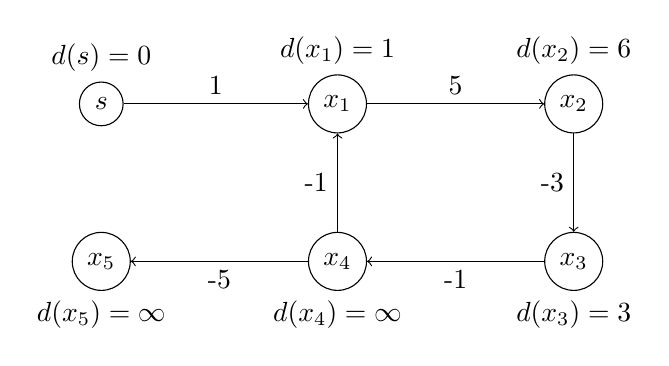
\begin{tikzpicture}[state/.style={draw, circle, fill=none,text centered, text=black}]
                        \node[state, label={$ d(s) = 0 $}] (s) at (0, 2) {$s$};
                        \node[state, label={$ d(x_1) = 1 $}] (x1) at (3, 2) {$x_1$};
                        \node[state, label={$ d(x_2) = 6 $}] (x2) at (6, 2) {$x_2$};
                        \node[state, label={-90:$ d(x_3) = 3 $}] (x3) at (6, 0) {$x_3$};
                        \node[state, label={-90:$ d(x_4) = \infty $}] (x4) at (3, 0) {$x_4$};
                        \node[state, label={-90:$ d(x_5) = \infty $}] (x5) at (0, 0) {$x_5$};
                        \draw [->] (s) -- node[anchor=south] {1} (x1);
                        \draw [->] (x1) -- node[anchor=south] {5} (x2);
                        \draw [->] (x2) -- node[anchor=east] {-3} (x3);
                        \draw [->] (x3) -- node[anchor=north] {-1} (x4);
                        \draw [->] (x4) -- node[anchor=north] {-5} (x5);
                        \draw [->] (x4) -- node[anchor=east] {-1} (x1);
                        \end{tikzpicture}
                    }
                \caption{$ \Gamma $}
                \end{figure}
            \end{column}
            \hfill
            \begin{column}{.48\textwidth}
                \begin{figure}[htb]
                    \resizebox {\linewidth} {!} {
                        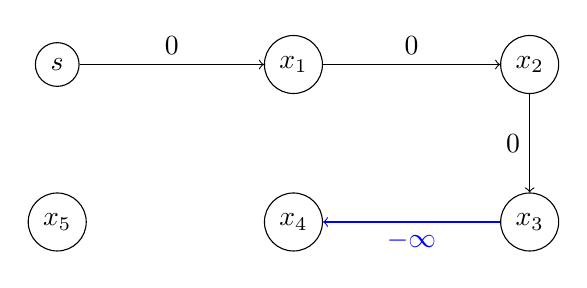
\begin{tikzpicture}[state/.style={draw, circle, fill=none, text centered, text=black}]
                        \node[state] (s) at (0, 2) {$s$};
                        \node[state] (x1) at (3, 2) {$x_1$};
                        \node[state] (x2) at (6, 2) {$x_2$};
                        \node[state] (x3) at (6, 0) {$x_3$};
                        \node[state] (x4) at (3, 0) {$x_4$};
                        \node[state] (x5) at (0, 0) {$x_5$};
                        \draw [->] (s) -- node[anchor=south] {0} (x1);
                        \draw [->] (x1) -- node[anchor=south] {0} (x2);
                        \draw [->] (x2) -- node[anchor=east] {0} (x3);
                        \draw [->, color=blue] (x3) -- node[anchor=north] {$ -\infty $} (x4);
                        \end{tikzpicture}
                    }
                    \caption{$ \Gamma_d $}
                \end{figure}
            \end{column}
        \end{columns}
        \begin{equation*}
                r(x,y) = weight(x,y) + d(x) - d(y)
        \end{equation*}
        \begin{center}
            \begin{tabular}{c c c}
                $ r(s,x_1) = 0 $ & $ r(x_1,x_2) = 0 $ & $ r(x_2,x_3) = 0 $ \\
                $ r(x_3,x_4) = -\infty $ & $ r(x_4,x_1) = \infty $ & $ r(x_4,x_5) = \varnothing $ \\
            \end{tabular}
        \end{center}
        $ \Gamma_d $ has no cycles. Let us relax the edge
        \textcolor{blue}{$ (x_3, x_4) $}
    \end{frame}




    \begin{frame}
        \frametitle{How to Find a Negative Cycle in a Graph}
        \begin{columns}[T]
            \begin{column}{.48\textwidth}
                \begin{figure}[htb]
                    \resizebox {\linewidth} {!} {
                        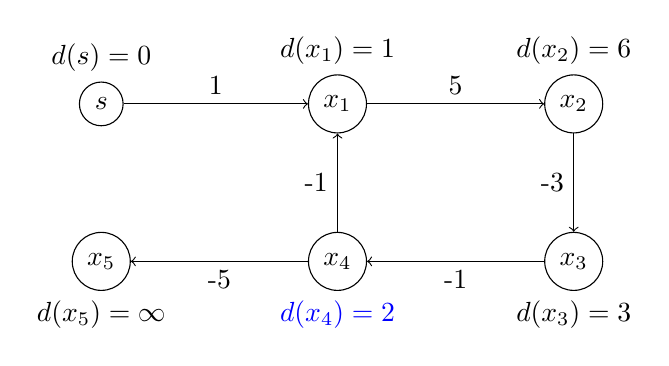
\begin{tikzpicture}[state/.style={draw, circle, fill=none,text centered, text=black}]
                        \node[state, label={$ d(s) = 0 $}] (s) at (0, 2) {$s$};
                        \node[state, label={$ d(x_1) = 1 $}] (x1) at (3, 2) {$x_1$};
                        \node[state, label={$ d(x_2) = 6 $}] (x2) at (6, 2) {$x_2$};
                        \node[state, label={-90:$ d(x_3) = 3 $}] (x3) at (6, 0) {$x_3$};
                        \node[state, label={-90:$ \textcolor{blue}{d(x_4) = 2} $}] (x4) at (3, 0) {$x_4$};
                        \node[state, label={-90:$ d(x_5) = \infty $}] (x5) at (0, 0) {$x_5$};
                        \draw [->] (s) -- node[anchor=south] {1} (x1);
                        \draw [->] (x1) -- node[anchor=south] {5} (x2);
                        \draw [->] (x2) -- node[anchor=east] {-3} (x3);
                        \draw [->] (x3) -- node[anchor=north] {-1} (x4);
                        \draw [->] (x4) -- node[anchor=north] {-5} (x5);
                        \draw [->] (x4) -- node[anchor=east] {-1} (x1);
                        \end{tikzpicture}
                    }
                    \caption{$ \Gamma $}
                \end{figure}
            \end{column}
            \hfill
            \begin{column}{.48\textwidth}
                \begin{figure}[htb]
                    \resizebox {\linewidth} {!} {
                        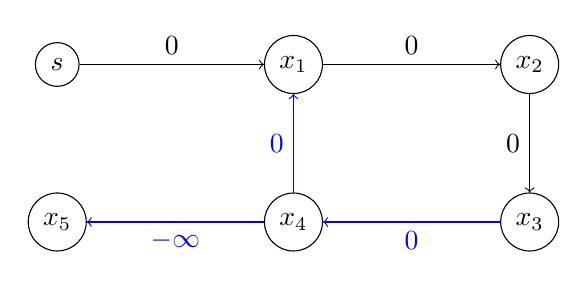
\begin{tikzpicture}[state/.style={draw, circle, fill=none, text centered, text=black}]
                        \node[state] (s) at (0, 2) {$s$};
                        \node[state] (x1) at (3, 2) {$x_1$};
                        \node[state] (x2) at (6, 2) {$x_2$};
                        \node[state] (x3) at (6, 0) {$x_3$};
                        \node[state] (x4) at (3, 0) {$x_4$};
                        \node[state] (x5) at (0, 0) {$x_5$};
                        \draw [->] (s) -- node[anchor=south] {0} (x1);
                        \draw [->] (x1) -- node[anchor=south] {0} (x2);
                        \draw [->] (x2) -- node[anchor=east] {0} (x3);
                        \draw [->, color=blue] (x3) -- node[anchor=north] {$ \textcolor{blue}{0} $} (x4);
                        \draw [->, color=blue] (x4) -- node[anchor=north] {$ \textcolor{blue}{-\infty} $} (x5);
                        \draw [->, color=blue] (x4) -- node[anchor=east] {\textcolor{blue}{0}} (x1);
                        \end{tikzpicture}
                    }
                    \caption{$ \Gamma_d $}
                \end{figure}
            \end{column}
        \end{columns}
        \begin{equation*}
            r(x,y) = weight(x,y) + d(x) - d(y)
        \end{equation*}
        \begin{center}
            \begin{tabular}{c c c}
                $ r(s,x_1) = 0 $ & $ r(x_1,x_2) = 0 $ & $ r(x_2,x_3) = 0 $ \\
                $ \textcolor{blue}{r(x_3,x_4) = 0} $ & $ \textcolor{blue}{r(x_4,x_1) = 0} $ & $ \textcolor{blue}{r(x_4,x_5) = -\infty} $ \\
            \end{tabular}
        \end{center}
        Now $ \Gamma_d $ has a cycle:
        \textcolor{blue}{$ x_1 \rightarrow x_2 \rightarrow x_3 \rightarrow x_4 \rightarrow x_1 $}.
        This cycle in $ \Gamma $ has indeed zero weight.
    \end{frame}



    \begin{frame}
        \frametitle{How to Find a Negative Cycle in a Graph}
        \begin{theorem}
            \label{the:neg-cycle-in-cg}
            Given a constraint graph $ \Gamma $ and a series of distance estimating
            functions $ (d_0, d_1, d_2, d_3, \dots) $, $ \Gamma $ has a negative
            or zero cycle if and only if $ \Gamma_d $ has a cycle under some
            distance estimate $ d_k $.
            \begin{proof}
                Use ``proof-by-contradiction`` approach.
                \\
                $ \Rightarrow $ Use the following fact inferred
                from~\textcolor{blue}{[Cormen \etal 2009]}.
                When $ \Gamma $ has
                a negative cycle then the series
                $ (d_0, d_1, d_2, d_3, \dots) $
                will \textcolor{blue}{never converge}.
                \\
                $ \Leftarrow $ Cycle is in $ \Gamma_d $
                therefore all its edges are
                \textcolor{blue}{admissible}
                and therefore
                $ d(x_i) + weight(x_i, x_{i+1}) \le d(x_{i+1}) $.
                Sum the latter inequality along all the edges of the
                cycle and show that the cycle's weight will be
                non-positive:
                $ \sum_{i=0}^{n-1} weight(x_i, x_{i+1}) \le 0 $
                \\
                For the full proof please see my seminar paper
                or~\textcolor{blue}{[Cotton~\etal~2004]}.
            \end{proof}
        \end{theorem}
    \end{frame}



    \begin{frame}
        \frametitle{Goldberg-Radzik Heuristic}
        \begin{itemize}
            \item \textcolor{blue}{[Goldberg+Radzik 1993]} suggests
            a heuristic to speed up Bellman-Ford algorithm
            in \textcolor{blue}{practical cases}.
            \item The theoretical upper bound stays the same:
            $ O(|V| \cdot |E|) $
            \item Idea:
            \begin{itemize}
                \item Mark vertices as ``unreached``, ``labeled``
                and ``scanned`` (vertex status)
                \item In the beginning of each \textcolor{blue}{pass}
                take vertices that have at least one outgoing admissible
                edge -- set $ B $
                \item Also, mark those vertices that have no outgoing
                admissible edges as ``scanned``
                \item Calculate set $ A $ -- unexplored vertices
                (\ie ``unreached``) which are reachable from $ B $
                in \textcolor{blue}{$ \Gamma_d $}
                \item \textcolor{blue}{Sort $ A $ topologically using
                $ \Gamma_d $
                as the input graph}
                \item Execute a \textcolor{blue}{pass}:
                \begin{itemize}
                    \item For each vertex in $ A $ relax all
                    outgoing admissible edges (of course, if they
                    can be relaxed \ie if $ r(x,y) < 0 $)
                \end{itemize}
                \item Execute passes until all the vertices are scanned
            \end{itemize}
        \end{itemize}
    \end{frame}



    \begin{frame}
        \frametitle{SAT Checking Algorithm for Difference Logic (Sketch)}
        \begin{figure}[htb]
            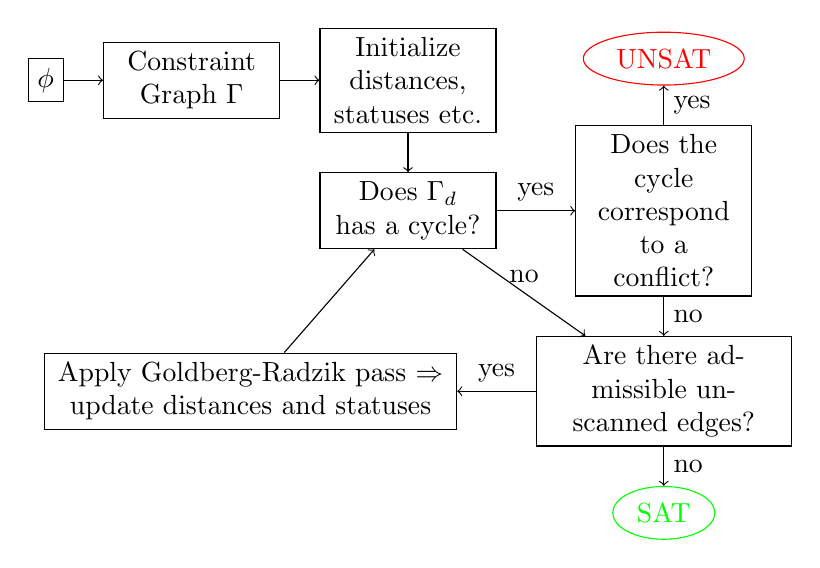
\begin{tikzpicture}
            \tikzstyle{block} = [draw, rectangle]
            \node [block] (formula) {$ \phi $};
            \node [block, right = 0.5cm of formula, text width=2cm, align=center] (cg) {Constraint Graph $ \Gamma $};
            \node [block, right = 0.5cm of cg, text width=2cm, align=center] (init1) {Initialize distances, statuses \etc};
            \node [block, below = 0.5cm of init1, text width=2cm, align=center] (checkCycle) {Does $ \Gamma_d $ has a cycle?};
            \node [block, right = of checkCycle, text width=2cm, align=center] (hasCycle) {Does the cycle correspond to a conflict?};
            \node [draw, ellipse, color=red, above = 0.5cm of hasCycle] (unsat) {UNSAT};
            \node [block, below = 0.5cm of hasCycle, text width=3cm, align=center] (admissibleEdges) {Are there admissible unscanned edges?};
            \node [draw, ellipse, color=green, below = 0.5cm of admissibleEdges] (sat) {SAT};
            \node [block, left = 1cm of admissibleEdges, text width=5cm, align=center] (applyGR) {Apply Goldberg-Radzik pass $ \Rightarrow $ update distances and statuses};

            \draw[->] (formula) -- (cg);
            \draw[->] (cg) -- (init1);
            \draw[->] (init1) -- (checkCycle);
            \draw[->] (checkCycle) -- node[anchor=south] {yes} (hasCycle);
            \draw[->] (checkCycle) -- node[anchor=south] {no} (admissibleEdges);
            \draw[->] (hasCycle) -- node[anchor=west] {yes} (unsat);
            \draw[->] (hasCycle) -- node[anchor=west] {no} (admissibleEdges);
            \draw [->] (admissibleEdges) -- node[anchor=west] {no} (sat);
            \draw [->] (admissibleEdges) -- node[anchor=south] {yes} (applyGR);
            \draw [->] (applyGR) -- (checkCycle);
            \end{tikzpicture}
        \end{figure}
    \end{frame}



    \begin{frame}
        \frametitle{Conclusion}
        \begin{itemize}
            \item Many timing problems (logistics, planning, scheduling,
            circuits checking) can be expressed in DL.
            Therefore it is important to have an efficient algorithm
            for checking SAT of a DL formula.
            \item Conjunction of DL constraints can be represented
            by a constraint graph $ \Gamma $.
            \begin{itemize}
                \item A negative cycle corresponds to a conflict
                $ 0 \prec c $ where $ c < 0 $
                and $ \prec \in \{ <, \le \} $.
                \item A zero weight cycle with a strict inequality
                edge corresponds to a conflict
                $ 0 < 0 $.
            \end{itemize}
            \item There is no need to enumerate all cycles in $ \Gamma $.
            Bellman-Ford algorithm can be used to detect a negative
            cycle in~$ O(|V| \cdot |E|) $ operations.
            \item A cycle in admissible graph $ \Gamma_d $
            corresponds to a negative or zero weight cycle in
            the corresponding constraint graph $ \Gamma $.
        \end{itemize}
    \end{frame}



    \begin{frame}
        \frametitle{Thank you}
        \Huge Thank you for your attention
    \end{frame}
\end{document}